\documentclass[a4j]{jsarticle}
\usepackage{graphicx}
\usepackage{listings}

\title{2024年度プログラミング\textsc{iii} 演習課題}
\author{学籍番号: 35714121 \\ 氏名: 福富隆大}
\date{2024年12月17日}

\begin{document}
\maketitle

\textbf{1 はじめに} \\

本レポートは演習課題第8~11回の実行結果をまとめたものである。\\

\textbf{2 課題} \\

\textmd{(題名)} \\

ギリギリになって焦って作ったRPGゲーム \\

\textmd{どのような技術を使ったか} 

制御構文の利用,関数(自作)の利用,ポインタの利用,構造体の利用,ファイル操作を使用して作った。 \\

\textmd{実行例} 

\begin{figure}[htbp]
  \centering 
  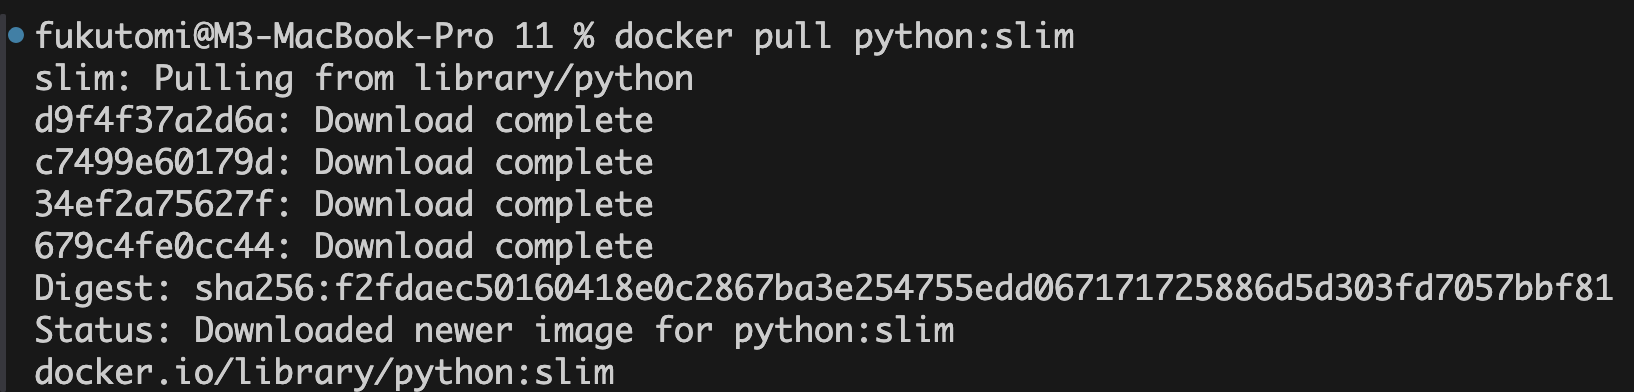
\includegraphics[width=10cm]{1.eps}
\end{figure}
\begin{figure}[htbp]
  \centering 
  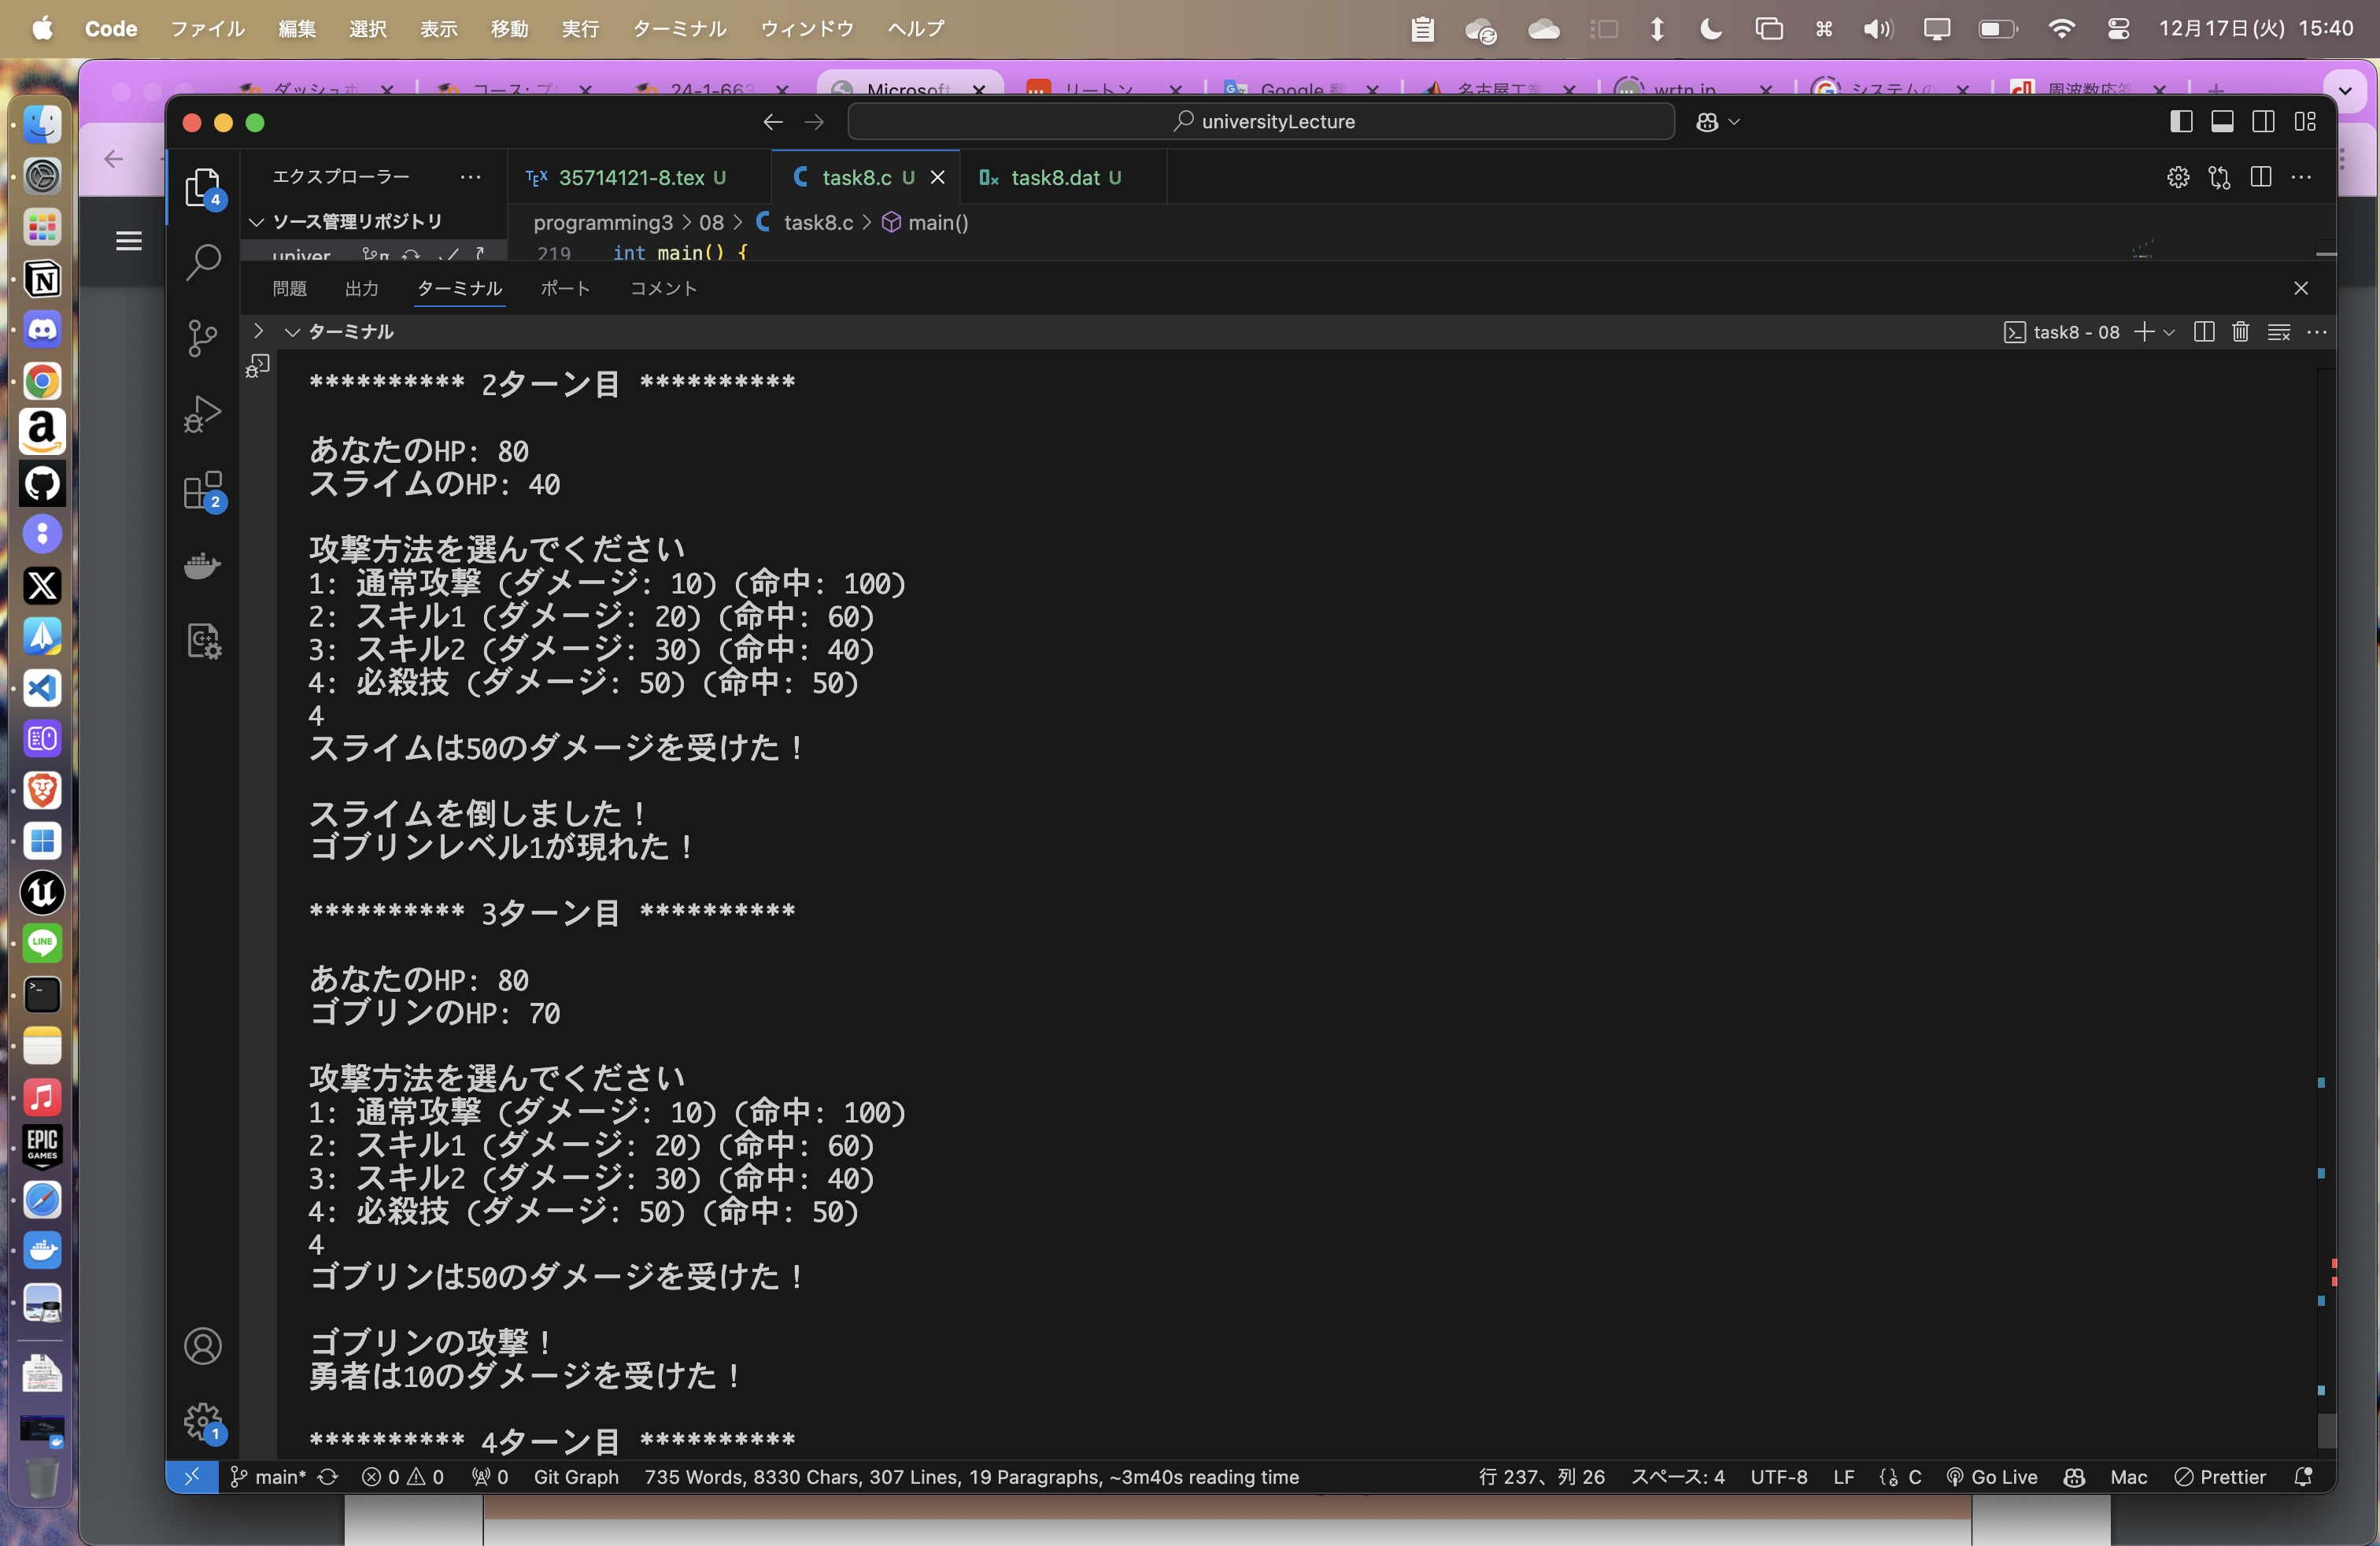
\includegraphics[width=10cm]{2.eps}
\end{figure}
\begin{figure}[htbp]
  \centering 
  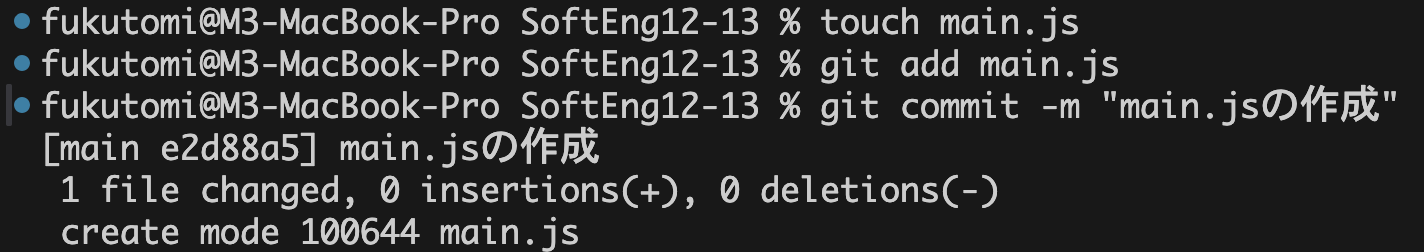
\includegraphics[width=10cm]{3.eps}
\end{figure}
\begin{figure}[htbp]
  \centering 
  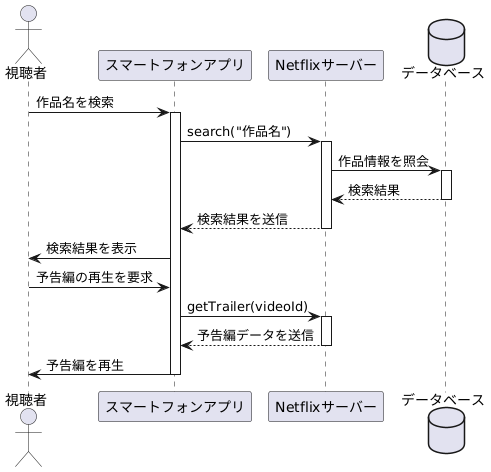
\includegraphics[width=10cm]{4.eps}
\end{figure}
\begin{figure}[htbp]
  \centering 
  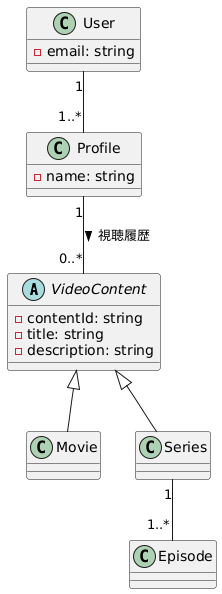
\includegraphics[width=10cm]{5.eps}
\end{figure}

\textmd{プログラムの解説} 

ライブラリはtdio.h,stdlib.h,time.hなどを使用した。\\
コンパイル方法は特に変わらず、gcc task8.c -o task8でコンパイルした。\\
プログラム動作の流れは
1. セーブデータがあれば読み込むか確認し、なければ初期データを使う。\\
2. 自分のHPかすべての敵のHPが0になるまで戦闘を繰り返す。\\
3. 自分の攻撃は攻撃方法を4択で選び、敵のHPを減らす。\\
4. 敵の攻撃はランダムで選ばれ、自分のHPを減らす。\\
5. 自分のHPが0になるとゲームオーバー、すべての敵のHPが0になるとクリア。\\
6. 敵を倒すと経験値が入り、一定値を超えるとレベルアップする。\\
7. セーブデータを作成するか確認し、作成すると次回からそのデータを使うことができる。\\

\textmd{感想} 
セーブデータの作成に時間がかかった。ポインタを使う部分の処理が思った通りにならないことが多く、どこが違うのかを探すのに時間がかかった。
敵モンスターの強さを選べたり、必殺技をチャージが必要にするなどの機能も追加したい。

\end{document}
